\documentclass[12pt]{amsart}

% PACKAGES
\usepackage[top=.5in, bottom=.5in, left=.7in, right=.7in]{geometry}
\usepackage{amsmath}        % AMS fonts and symbols
\usepackage{amsthm}         % Theorems in AMS style
\usepackage{amssymb}        % Additional AMS symbols
\usepackage{amsfonts}       % Additional AMS fonts
\usepackage{amsthm}			% Theorems, remarks, etc
\usepackage{bbm}			% Blackboard bold numbers
\usepackage{nicefrac}       % Partially stacks horizontal fractions
\usepackage{scrextend}      % Required to manipulate margins
\usepackage{mathrsfs}       % Adds \mathscr, i.e. math script style
\usepackage{hyperref}       % Displays hyperlinks
\usepackage{enumitem}       % Additional enumeration features
\usepackage{verbatim}       % Displays code-like text
\usepackage{graphicx}       % Used for graphics
\usepackage{cite}           % Enables bibtex bibliographies
\usepackage{soul}           % Special text editing, for MP comments
\usepackage{color}
  
% PAGE LAYOUT
\setlength{\parskip}{\baselineskip}
\setlength\parindent{0pt}

\begin{document}
\section{Sample Problem}
\section{Classical Form}
Let $\Omega = (0,1) \times (0,1) \subset \mathbb{R} \times \mathbb{R}$, let
$\Gamma = \partial \Omega$, and define 
%
\begin{subequations}
	\label{eq:example1-1}
\begin{eqnarray}
	\label{eq:example1-1a}
	\Gamma_1 &:=& \{(x,y) \in \partial \Omega : 0 < x < 1, y = 0 \} \\
	%
	\label{eq:example1-1b}
	\Gamma_2 &:=& \{(x,y) \in \partial \Omega : x = 1, 0 < y < 1 \} \\
	%
	\label{eq:example1-1c}
	\Gamma_3 &:=& \{(x,y) \in \partial \Omega : 0 < x < 1, y = 1 \} \\
	%
	\label{eq:example1-1d}
	\Gamma_4 &:=& \{(x,y) \in \partial \Omega : x = 0, 0 < y < 1 \}
\end{eqnarray}
\begin{subequations}
%
Let 
%
\begin{subequations}
\label{eq:example1-2} 
\begin{eqnarray}
	\label{eq:example1-2a}
	\Gamma_{ij} &:=& \overline{\Gamma}_i \cup \overline{\Gamma}_j, \{1 \leq i < j \leq 4 \} \\ 
	%
	\label{eq:example1-2b}
	\Gamma_{ijk} &:=& \overline{\Gamma}_i \cup \overline{\Gamma}_j \cup \overline{\Gamma}_k,
	\{1 \leq i < j < k \leq 4 \} \\
	%
	\label{eq:example1-2c}
	\mathring{\Gamma}_{ij} &:=& \Gamma \setminus \Gamma_{k\ell}, 
	\text{ where } \{k, \ell\} := \{1, 2, 3, 4\} \setminus \{i, j\} \\
	%
	\label{eq:example1-2d}
	\mathring{\Gamma}_{ijk} &:=& \Gamma \setminus \Gamma_{\ell}, 
	\text{ where } \{\ell\} := \{1,2,3,4\} \setminus \{i, j, k\}.
\end{eqnarray}
\end{subequations}
%
Throughout, we will consider the following example problem: Given $f \in
L^2(\Omega)$, $u_D \in H^1(\Omega)$, and $g \in L^2(\Gamma_N)$, seek $u \in
H^1(\Omega)$ such that
%
\begin{subequations}
	\label{eq:example1-3}
\begin{eqnarray}
	\label{eq:example1-3a
	-\nabla u &=& f, \text{ in } \Omega \\
	%
	\label{eq:example1-3b
	u &=& u_D, \text{ on } \Gamma_D \\
	%
	\label{eq:example1-3c
	-\grad u \cdot n &=& g \text{ on } \Gamma_N,		
\end{eqnarray}
\end{subequations}
%
where $\Gamma_D \cup \Gamma_N = \Gamma$, $\Gamma_D \cap \Gamma_N =
\varnothing$, and each of $\Gamma_D, \Gamma_N$ is defined per
\eqref{eq:example1-2}, or is empty. 

In \eqref{eq:example1-3}, $n$ is the unit outward normal vector to $\Gamma$,
which is defined only where $\Gamma$ is regular enough; i.e. $n$ is not defined
on the corners of $\Gamma$, and so is only defined almost everywhere on
$\Gamma$. Nevertheless, when considering the weak formulation of
\eqref{eq:example1-3}, to be described below, $n$ need only be defined almost
everywhere on $\Gamma$ in order for definition \eqref{eq:example1-3c} to make
sense. 


\subsection{Weak Formulation}
If the Dirichlet conditions given by \eqref{eq:example1-3b} are inhomogeneous,
then they are incorporated through the decomposition $v = u - u_D$ so that $v =
0$ on $\Gamma_D$, i.e. 
%
\begin{eqnarray}
	\label{eq:example1-4}
	v \in H^1_D(\Omega) := \{ w \in H^1(\Omega) : w = 0 \text{ on } \Gamma_D \}.
\end{eqnarray}
%
The weak formulation of \eqref{eq:example1-3} is then to seek $v \in
H^1_D(\Omega)$ such that 
%
\begin{eqnarray}
	\label{eq:example1-5}
	\int_{\Omega} \nabla v \cdot \nabla w dx
	= \int_{\Omega} fw dx + \int_{\Gamma_N} gw ds - \int_\Omega \nabla u_D \cdot \nabla w dx, 
	\qquad w \in H^1_D(\Omega).
\end{eqnarray}
%
Observe therefore that $g$ need only be defined almost everywhere on
$\Gamma_N$. Thus, if $\Gamma_N$ contains one or more corners, so that $n$ is
undefined at some finite number of points of $\Gamma_N$, the boundary condition
\eqref{eq:example1-3c}, which appears in \eqref{eq:example1-5} as the term
$int_{\Gamma_N} gw ds$, still makes sense.


\subsection{Domain Discretization} 
For each $h > 0$, the domain $\overline{\Omega}$ is subdivided into $N_h$-many
triangles $\mathcal{T} = \{T_i\}_{i=1}^{N_h}$ such that $\overline{\bigcup_{1
\leq i \leq N_h} T_i} = \overline{\Omega}$, $T_i \cap T_j = \varnothing$ for $i
\neq j$, $\text{diam } T_i < h$ for $1 \leq i \leq N_h$, and such that the
angles of all $T_i \in \mathcal{T}$ are uniformly bounded away from zero. 

Throughout, we will set $h = \tfrac{1}{2}$ and use the triangulation depicted
in figure \ref{fig:example1-1} in our examples. The coordinates of the nodes in
this example are given in table \ref{tab:example1-1}. 

%
\begin{figure}[h!]
	\includegraphics[width=0.5\linewidth]{triangulated_domain.png}
	\caption{}
	\label{fig:example1-1}
\end{figure}
%

%
\begin{table}[h!]
    \centering
    \begin{tabular}{c c c}
    \hline
		\textbf{node} & \textbf{x-coord.} & \textbf{y-coord.}
	\hline
		1	&	0 		& 0			\\
		2	&	1 		& 0			\\
		3	&	1 		& 1			\\
		4	&	0 		& 1			\\
		5	&	0 		& 0.5		\\
		6	&	0.5 	& 0			\\
		7	&	0.5 	& 1			\\
		8	&	1 		& 0.5		\\
		9	&	0.6449 	& 0.6449	\\
		10	&	0.7019 	& 0.2975	\\
		11	&	0.2975 	& 0.7019	\\
		12	&	0.3480 	& 0.3480	\\
	\hline
    \end{tabular}
    \caption{Coordinates for nodes in example triangulation.}
    \label{tab:example1-1}
\end{table}
%


\section{Dirichlet Conditions}
\subsection{Homogeneous Dirichlet Condition} 
For problem \eqref{eq:example1-3} with $\Gamma_N = \varnothing$ and $u_D = 0$
on $\Gamma_D = \Gamma$. Then the space of test functions is 
%
\begin{eqnarray}
	\label{eq:dirichlet1-1}
	H^1_D(\Omega) := \{w \in H^1(\Omega) : w = 0 \text{ on } \Gamma\} = H^1_0(\Omega).
\end{eqnarray}
%
So, in the weak formulation \eqref{eq:example1-5}, the term $\int_\Gamma gw ds
= 0$ because $w = 0$ on $\Gamma$. Thus, that term drops out of the computation.
Additionally, the term $\int_\Omega \nabla u_D \cdot \nabla w dx = 0$ because
$u_D = 0$ on $\Omega$, so also $\nabla u_D = 0$ on $\Omega$; so that term drops
out as well. 


\subsection{Inhomogeneous Dirichlet Condition}
Now consider problem \eqref{eq:example1-3} with $\Gamma_N = \varnothing$ but
with $u_D \neq 0$ on some nontrivial part of $\Gamma$. This inhomogeneous
Dirichlet condition is incorporated by decomposing $u = v + u_D$ where $v = 0$
on $\Gamma_D = \Gamma$, i.e. $v \in H_0^1(\Omega)$. So, again, the test space
is $H_0^1(\Omega)$, meaning that in the weak formulation \eqref{eq:example1-5},
the term $\int_\Gamma gw ds = 0$, because again $w = 0$ on $\Gamma$. This time,
however, the term $u_D \neq 0$, so $\nabla u_D$ is not necessarily zero, so the
term $\int_\Omega \nabla u_D \cdot \nabla w dx$ is no longer necessarily zero.
However, because $u_D$ is given, the term $\int_\Omega \nabla u_D \cdot \nabla
w dx$ may be moved over to the right hand side, where it acts as an additional
source. The problem is now reduced to finding $v$, subject to this additional
source term; once $v$ is known, the solution may be recovered as $u = v + u_D$. 


\subsection{Handling Inhomogeneous Dirichlet Conditions: A Naive Approach}
Suppose that in \eqref{eq:example1-3}, $\Gamma_N = \varnothing$ and $u_D = c$
on $\Gamma_D = \Gamma$ where $c \in \mathbb{R}$. Then one might naively define
$u_D = c$ on all of $\Omega$. In this case, $\grad u_D = 0$, so that the term
$\int_\Omega \grad u_D \cdot \grad w dx = 0$ as well. In this context, the
decomposition $u = v + u_D$ suggests to solve \eqref{eq:example1-3} by summing
the solution to two subproblems: The term $v$ solves the problem 
%
\begin{subequations}
	\label{eq:dirichlet1-2}
\begin{eqnarray}
	\label{eq:dirichlet1-2a}
	-\Delta v &=& f, \text{ in } \Omega \\
	%
	\label{eq:dirichlet1-2b}
	v &=& 0, \text{ on } \Gamma,
\end{eqnarray}
\end{subequations}
%
i.e. $v$ solves the problem with homogeneous Dirichlet conditions and an
inhomogeneous source. Then $u_D$ solves the problem 
%
\begin{eqnarray}
	\label{eq:dirichlet1-3}
	-\Delta u_D &=& 0, \text{ \in } \Omega
\end{eqnarray}
%
where, per \eqref{eq:example1-3b}, $u_D$ satisifes the desired inhomogeneous
Dirichlet boundary conditions. Thus $u_D$ satisifes the problem with
homogeneous source but inhomogeneous Dirichlet boundary condtions. Summing
\eqref{eq:dirichlet1-2a} and \eqref{eq:dirichlet1-3} gives 
%
\begin{eqnarray}
	\label{eq:dirichlet1-4}
	-\Delta v - \Delta u_D = - \Delta (v + u_D) = -\Delta u = f
\end{eqnarray}
%
and the desired boundary conditions are satisified because of
\eqref{eq:dirichlet1-2b}, i.e. because $u = v + u_D = u_D$ on $\Gamma$.

Let us also demonstrate this naive approach numerically. Using the Galerkin approach
on the triangulation defined in table \ref{tab:example1-1}, problem
\eqref{eq:dirichlet1-2} reduces to $SV = B$ where 
%
\begin{eqnarray}
	\label{eq:dirichlet1-5}
	S =
	\begin{bmatrix}
		1 &  &  &  &  &  &  &  &  &  &  &  \\
		 & 1 &  &  &  &  &  &  &  &  &  &  \\
		 &  & 1 &  &  &  &  &  &  &  &  &  \\
		 &  &  & 1 &  &  &  &  &  &  &  &  \\
		 &  &  &  & 1 &  &  &  &  &  &  &  \\
		 &  &  &  &  & 1 &  &  &  &  &  &  \\
		 &  &  &  &  &  & 1 &  &  &  &  &  \\
		 &  &  &  &  &  &  & 1 &  &  &  &  \\
		 &  &  &  &  &  &  &  & 
				(\nabla \varphi_{9},  \nabla \varphi_{9}) & 
				(\nabla \varphi_{10}, \nabla \varphi_{9}) & 
				(\nabla \varphi_{11}, \nabla \varphi_{9}) & 
				(\nabla \varphi_{12}, \nabla \varphi_{9}) \\
		 &  &  &  &  &  &  &  & 
				(\nabla \varphi_{9},  \nabla \varphi_{10}) & 
				(\nabla \varphi_{10}, \nabla \varphi_{10}) & 
				(\nabla \varphi_{11}, \nabla \varphi_{10}) & 
				(\nabla \varphi_{12}, \nabla \varphi_{10}) \\
		 &  &  &  &  &  &  &  & 
				(\nabla \varphi_{9},  \nabla \varphi_{11}) & 
				(\nabla \varphi_{10}, \nabla \varphi_{11}) & 
				(\nabla \varphi_{11}, \nabla \varphi_{11}) & 
				(\nabla \varphi_{12}, \nabla \varphi_{11}) \\
		 &  &  &  &  &  &  &  & 
				(\nabla \varphi_{9},  \nabla \varphi_{12}) & 
				(\nabla \varphi_{10}, \nabla \varphi_{12}) & 
				(\nabla \varphi_{11}, \nabla \varphi_{12}) & 
				(\nabla \varphi_{12}, \nabla \varphi_{12}) \\
	\end{bmatrix},
	\qquad
	B = 
	\begin{bmatrix}
		0 \\
		0 \\
		0 \\
		0 \\
		0 \\
		0 \\
		0 \\
		0 \\
		(f, \varphi_{9})  \\
		(f, \varphi_{10}) \\
		(f, \varphi_{11}) \\
		(f, \varphi_{12}) \\
	\end{bmatrix}
\end{eqnarray}
%
This combination of $S$ and $B$ fixes the value of $V_i = 0$ for $i = \{1,
\dots, 8\}$, i.e. for the boundary nodes. Figure \ref{fig:dirichlet1-1} shows
the solution with this $S$ and $B$. It is clear that if this solution is
shifted up by $c$ units, then it will be the correct solution. And also, it is
clear that if $u_D = c$ on all of $\Omega$, then $u_D$ should be discretized as
$(U_D)_i = c$ for $i = \{1, \dots 12\}$, in which case the final solution $U =
V + U_D$ will literally be $V$ shifted up by $c$ units. 

%
\begin{figure}[h!]
	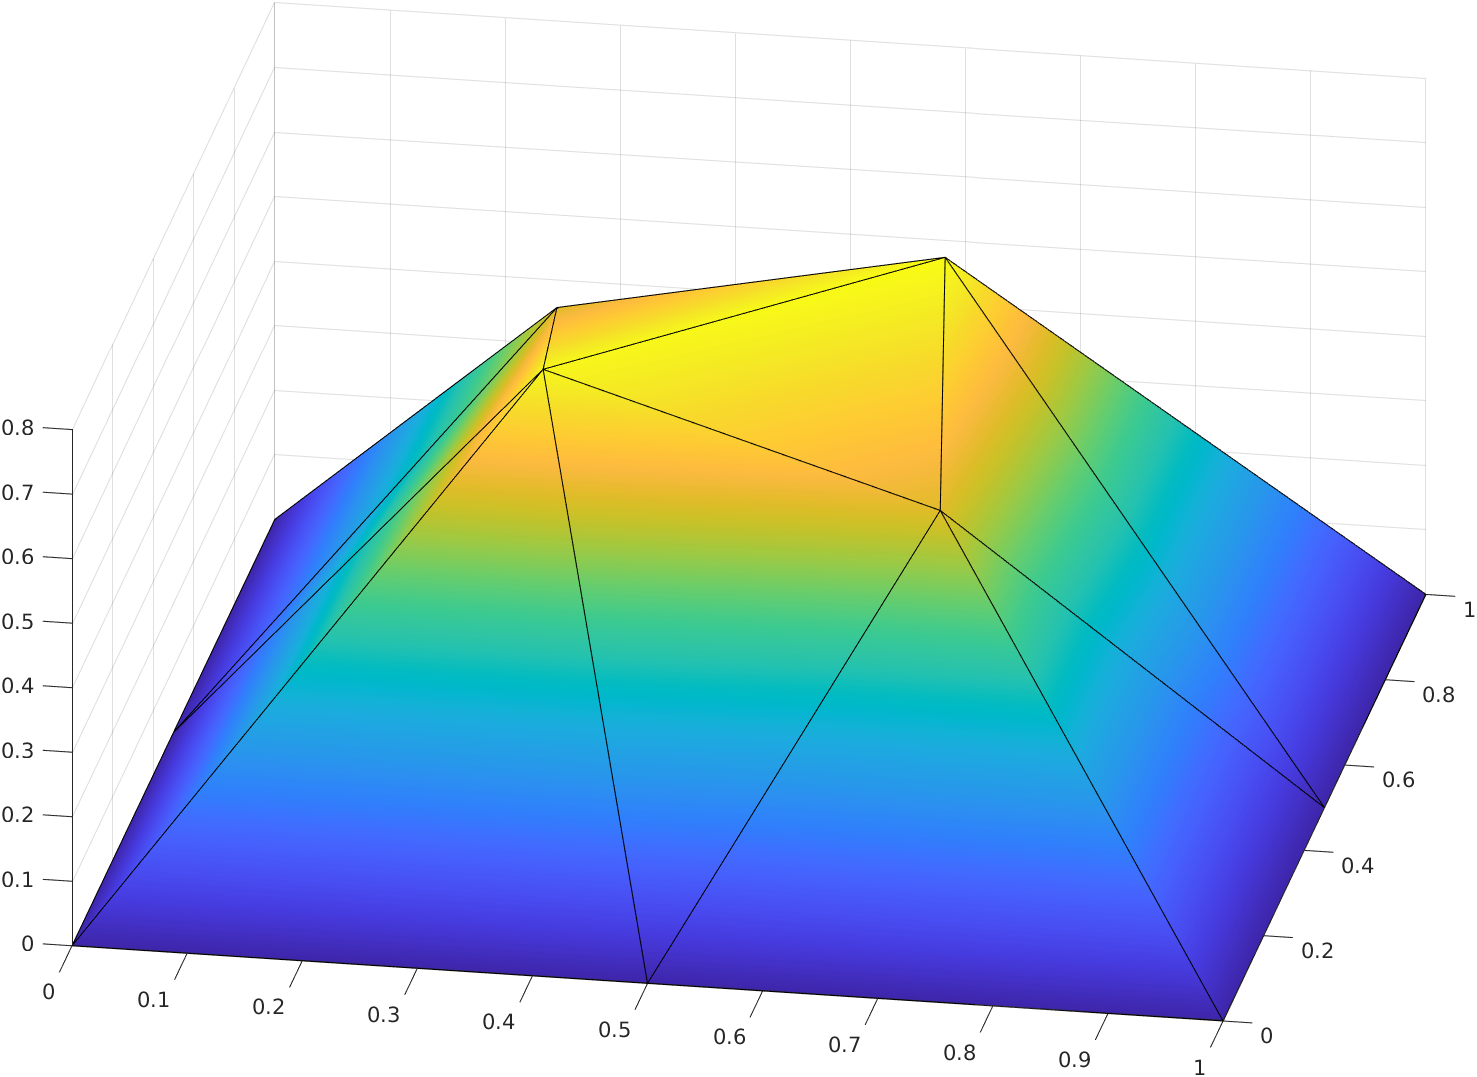
\includegraphics[width=0.4\linewidth]{BoundaryCondition_images/naive_dirichlet1.png}
	\caption{Solution with $S$ and $B$ given by \eqref{eq:dirichlet1-5}.}
	\label{fig:dirichlet1-1}
\end{figure}
%

To summarize, in the case where $u_D = c$ on $\Gamma$, it is tempting to set
$u_D = c$ throughout $\Omega$, and then simply find the solution $v$ to the
corresponding problem with homogeneous Dirichlet boundary conditions. This
approach is attractive because it is intuitive; one imagines decomposing a
problem with inhomogeneous source and inhomogeneous Dirichlet boundary
conditions into two subproblems: One with inhomogeneous source but homogeneous
boundary conditions, i.e. problem \eqref{eq:dirichlet1-2}, and one with
homogeneous source but inhomogeneous boundary conditions, i.e. problem
\eqref{eq:dirichlet1-3}. 

However, here is the problem: From the underlying theory, this approach
only works because $\nabla u_D = 0$, so that the term $\int_\Omega \nabla u_D
\cdot \nabla w dx = 0$ and therefore drops out of the weak formulation
\eqref{eq:example1-5}. For inhomogeneous Dirichlet boundary conditions that
are more complicated, it may not be possible to prescribe $u_D$ so that $\nabla
u_D = 0$ throughout $\Omega$. Thus, a more sophisticated approach is needed. 


\subsection{Handling Inhomogeneous Dirichlet Conditions: A Better Approach, part 1}
Let's jump to the discretized problem and, for sake of illustration, let $u_D =
1$ on $\Gamma$. Suppose $(x_i,y_i)$ are the coordinates of the $i$th node.
Let's choose $U_D$ so that $(U_D)_i = u_D(x_i,y_i)$ for $i = \{1, \dots, 8\}$
and $(U_D)_j = 0$ for $j = \{9, \dots, 12\}$. That is, $U_D$ should agree with
$u_D$ at the boundary nodes and be zero at all interior nodes. Figure
\ref{fig:dirichlet1-2} shows $U_D$.

%
\begin{figure}[h!]
	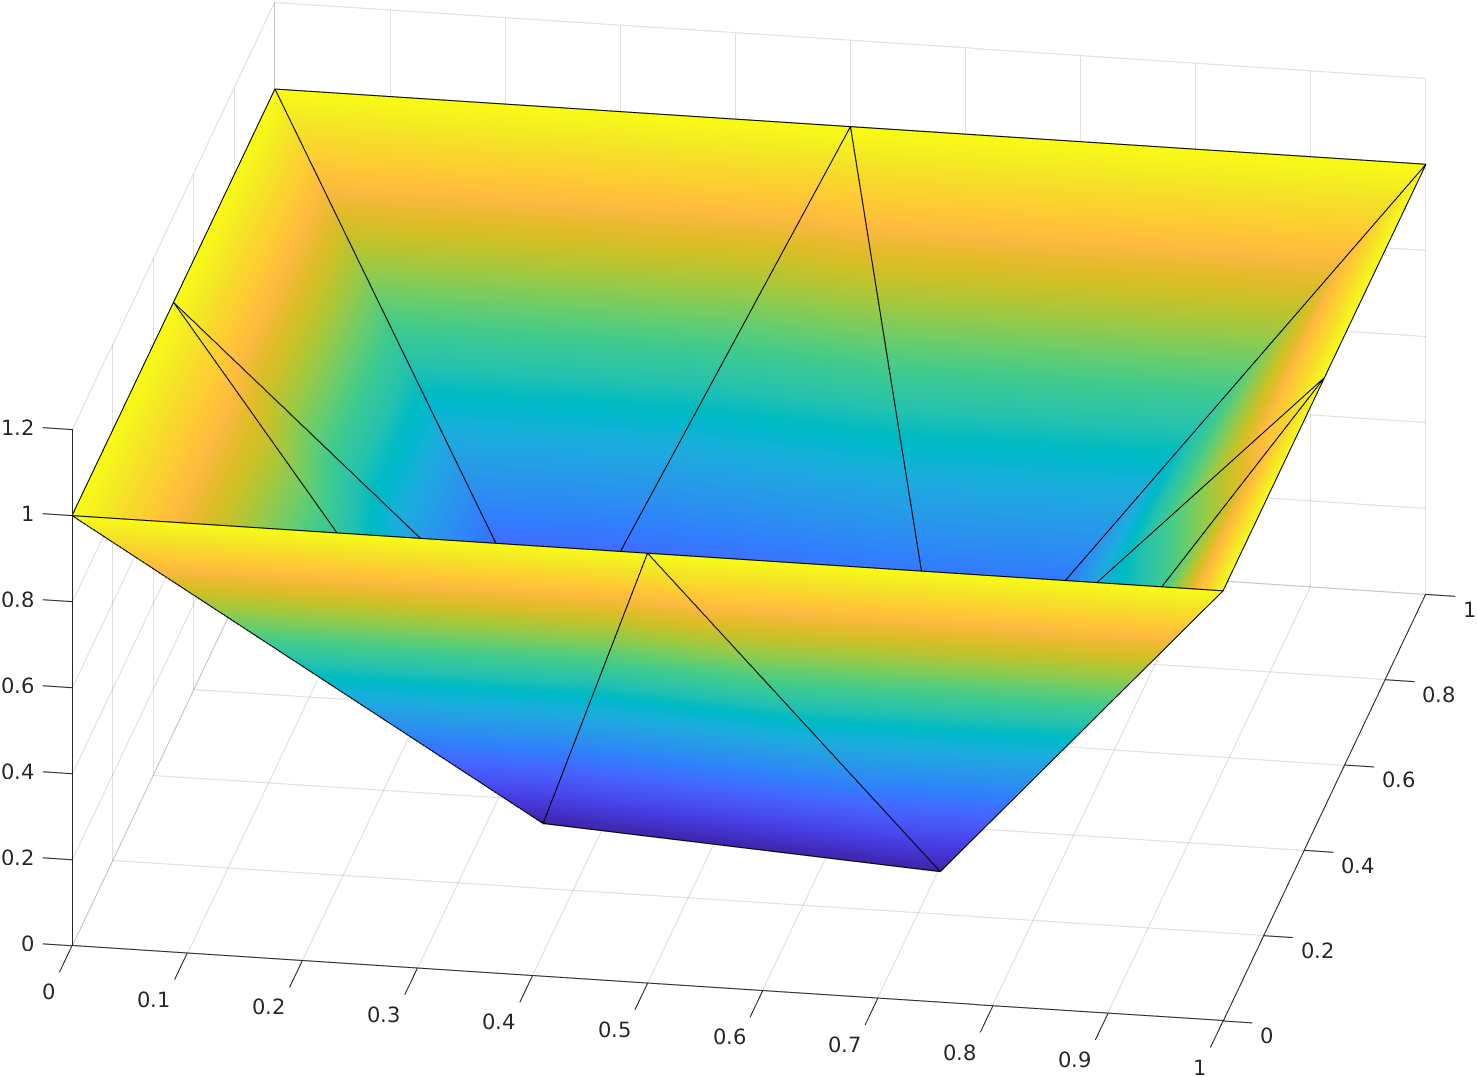
\includegraphics[width=0.4\linewidth]{BoundaryConditions_images/better_dirichlet1.png}
	\caption{$U_D$ for the improved approach.}
	\label{fig:dirichlet1-2}
\end{figure}
%

Now, it is clear that if $V$ is solved as the corresponding problem with
homogeneous dirichlet boundary conditions, as in the naive approach above, then
$U = V + U_D$ will be incorrect. In the naive approach, $U_D$ boosted the value
of $V$ on the interior nodes, and this allowed to solve $V$ using the same
source term as the original problem. However now, because $(U_D)_j = 0$ on
interior nodes, we cannot rely on $U_D$ to boost $V$ up to the correct value.
Instead, $V$ must attain the correct values on the interior nodes by itself.
Clearly this must be accomplished by increasing the value of the source term.
And, referring back to the weak formulation \eqref{eq:example1-5}, we see the
necessary source term is exactly the discretized version of $-\int_\Omega
\nabla u_D \cdot \nabla w dx$.

From figure \ref{fig:dirichlet1-2}, it is clear that $\nabla U_D \neq 0$ on any
triangle with an edge that coincides with $\Gamma$. Thus, we expect that $-\int
\nabla U_D \cdot \nabla \varphi_i \neq 0$ for any basis function $\varphi_i$
(i.e. hat function) such that node $i$ is either on $\Gamma$, or is connected
to a node on $\Gamma$. However, at the same time, recall that $v \in
H_0^1(\Omega)$. Thus, we will not include basis functions centered around
boundary nodes. Instead, we again use $S$ as in \eqref{eq:dirichlet1-5} and now
$B$ is given by 
%
\begin{eqnarray}
	\label{eq:dirichlet1-6}
	
\end{eqnarray}
%

\subsection{Integral Transforms for Triangles}
\subsubsection{Method}
To integrate over triangle $A$ with vertices $a = (a_1,a_2)$, $b = (b_1,b_2)$,
$c = (c_1,c_2)$, usually we employ a change of variables to instead integrate
over the standard reference triangle $\hat{A}$ defined by $\hat{a} = (0,0)$,
$\hat{b} = (1,0)$, $\hat{c} = (0,1)$.

Let $T: \hat{A} \to A$ defined by $T(\hat{x},\hat{y}) =
(x(\hat{x},\hat{y}),y(\hat{x},\hat{y}))$ where coordinate functions $x =
x(\hat{x},\hat{y})$ and $y = y(\hat{x},\hat{y})$ are one-to-one and $C^1$ and
where $T$ has nonzero Jacobian on the interior of region $\hat{A}$. Let $f$ be
a continuous function on $A$. Then 
%
\begin{eqnarray}
	\label{eq:transform_method1-1}
	\int_A f(x,y) dA 
	= \int_\hat{A} f(x(\hat{x},\hat{y}),y(\hat{x},\hat{y})) |J(\hat{x},\hat{y})| d\hat{x} d\hat{y}
\end{eqnarray}
%
where $J(\hat{x},\hat{y})$ is the Jacobian determinant of $T$.

In the case of transforming one triangle into another, transformation $T$ is
affine and can be computed using the formula 
%
\begin{eqnarray}
	\label{eq:transform_method1-2}
	\begin{bmatrix}
		a_1 & b_1 & c_1 \\
		a_2 & b_2 & c_2 \\
		1 & 1 & 1
	\end{bmatrix}
	=
	\begin{bmatrix}
		R_{11} & R_{12} & B_1 \\
		R_{21} & R_{22} & B_2 \\
		0 & 0 & 1
	\end{bmatrix}
	\begin{bmatrix}
		1 & 0 & 0 \\
		0 & 1 & 0 \\
		1 & 1 & 1
	\end{bmatrix}
\end{eqnarray}
%
or 
%
\begin{eqnarray}
	\label{eq:transform_method1-3}
	\bar{T} 
	:= 
	\begin{bmatrix}
		R_{11} & R_{12} & B_1 \\
		R_{21} & R_{22} & B_2 \\
		0 & 0 & 1
	\end{bmatrix}
	=
	\begin{bmatrix}
		a_1 & b_1 & c_1 \\
		a_2 & b_2 & c_2 \\
		1 & 1 & 1
	\end{bmatrix}
	\begin{bmatrix}
		1 & 0 & 1 \\
		0 & 1 & 1 \\
		1 & 1 & 1
	\end{bmatrix}^{-1}.
\end{eqnarray}
%
From $\bar{T}$, one obtains transformation $T$, the Jacobian determinant
$J(\hat{x},\hat{y})$, and the coordinate functions $x = x(\hat{x},\hat{y})$, $y
= y(\hat{x},\hat{y})$. To do so, observe that the submatrix $R$ defined by
$R_{ij}$ defines how the triangle is rotated and stretched. The column $B$
defined by $B_i$ defines how the triangle is translated. So $T$ is defined 
%
\begin{eqnarray}
	\label{eq:transform_method1-4}
	\begin{bmatrix} x \\ y \end{bmatrix}
	=
	T \left( \begin{bmatrix} \hat{x} \\ \hat{y} \end{bmatrix} \right) 
	:=
	R \begin{bmatrix} \hat{x} \\ \hat{y} \end{bmatrix} + B,
\end{eqnarray}
%
so that $J = \det(R)$ and $x = x(\hat{x},\hat{y})$ and $y = y(\hat{x},\hat{y})$
are the first and second rows of \eqref{eq:transform_method1-4}, respectively.

The above suggests the following method:
%
\begin{enumerate}
	\item Compute $\bar{T}$ from the vertex coordinates of $A$ and $\hat{A}$,
		per \eqref{eq:transform_method1-3}.
	%
	\item Compute and store $\begin{bmatrix} 1 & 0 & 0 \\ 0 & 1 & 0 \\ 1 & 1 & 1
		\end{bmatrix}^{-1}$.
	%	
	\item Compute coordinate functions $x = x(\hat{x},\hat{y})$, $y =
		y(\hat{x},\hat{y})$ and Jacobian determinant $J$, per
		\eqref{eq:transform_method1-4}.
	%	
	\item Use these to compute $\int_A f(x,y) dA$ per the coordinate transform
		given by \eqref{eq:transform_method1-1}.
\end{enumerate}



\subsubsection{Remarks}
In the previous subsection, hatted quantities refer to the reference triangle.
That is, $\hat{A}$ refers to the reference triangle itself; $\hat{a}$,
$\hat{b}$, $\hat{c}$ are the vertices of $\hat{A}$; and $(\hat{x},\hat{y})$ are
the coordinates of some point in $\hat{A}$. Un-hatted quantites refer to the
corresponding objects in the actual triangle $A$. Thus, the transformation 
%
\begin{eqnarray}
	\label{eq:transform_remarks1-1}
	T: (\hat{x},\hat{y}) \in \hat{A} \to A \ni (x,y) = (x(\hat{x},\hat{y}),y(\hat{x},\hat{y})
\end{eqnarray}
%
takes points $(\hat{x},\hat{y})$ in the reference triangle to points $(x,y)$ in
the actual triangle. 

As a sanity check: The function to be integrated on the left or right side of
\eqref{eq:transform_method1-1} is the function $f$. It's just that on the right
hand side of \eqref{eq:transform_method1-1}, we first take a point from the
reference triangle, map it to the corresponding point in the actual triangle,
and thereby obtain the same function value $f(x,y)$ that we would have obtained
had we just started in the reference triangle. From this perspective, you can
think of the right hand side of \eqref{eq:transform_method1-1} as pre-composing
$f$ with the transform that takes us from the reference triangle (which is the
region over which we \textit{want} to integrate) to the actual triangle (which
is the region over which we \textit{actually} integrate). 

As a second sanity check: The magnitude of the integral of a function is going
to be related to the magnitude of the area over which you integrate. But for an
affine transformation, we find that $J(\hat{x},\hat{y}) = J$ is a constant, and
that furthermore $J = |A| / |\hat{A}|$. So this factor corrects for the
difference in area of $A$ versus $\hat{A}$.

As a third sanity check, and a convenience of this method: Observe in
\eqref{eq:transform_method1-3} that the computation of $\bar{T}$ (and hence the
computation of $T$, $J$, and the coordinate functions) requires inverting a
matrix. For a grid with thousands of triangles, also thousands of $\bar{T}$'s
will have to be computed. However, in this method, it is the matrix of the
reference triangle that gets inverted, and the reference triangle is always the
same! So one can simply invert the matrix of the reference triangle \textit{once},
store that, and then the computation of each $\bar{T}$ amounts to a matrix
multiplication between known matrices. 

Finally, observe that in practice, the transformed integral is approximated
using Gaussian quadrature, which will be described elsewhere. By contrast, in
the following example, all integrals were computed by actually integrating.


\subsubsection{Example}
Consider the triangle $T$ defined by $a = (0.5,1)$, $b = (0.6449,0.6449)$, $c =
(1,1)$ and the function 
%
\begin{eqnarray}
	\label{eq:transform_example1-1}
	f(x,y) = x(x-1)y(y-1).
\end{eqnarray}
%
Then 
%
\begin{eqnarray}
	\label{eq:transform_example1-2}
	\int_T f(x,y) dA 
	= \int_{0.5}^{0.6449} \int_{-2.4516x + 2.2258}^1 x(x-1)y(y-1) dydx
	= 0.0018.
\end{eqnarray}
%
On the other hand, we compute $\bar{T}$ as 
%
\begin{eqnarray}
	\label{eq:transform_example1-3}
	\bar{T} := 
	\begin{bmatrix}
		R_{11} & R_{12} & B_1 \\
		R_{21} & R_{22} & B_2 \\
		0 & 0 & 1
	\end{bmatrix}
	=
	\begin{bmatrix}
		0.5 & 0.6449 & 1 \\
		1   & 0.6449 & 1 \\
		1   & 1      & 1
	\end{bmatrix}
	\begin{bmatrix}
		1 & 0 & 0 \\
		0 & 1 & 0 \\
		1 & 1 & 1
	\end{bmatrix}^{-1}
	=
	\begin{bmatrix}
		0.5 & -0.3551 & 1 \\
		0   & -0.3551 & 1 \\
		0   &       0 & 1
	\end{bmatrix}
\end{eqnarray}
%
implying that $T$ is defined 
%
\begin{eqnarray}
	\label{eq:transform_example1-4}
	T \left( \begin{bmatrix} \hat{x} \\ \hat{y} \end{bmatrix} \right) 
	= 
	\begin{bmatrix} 
		-0.5 & -0.3551 \\
		0    & -0.3551 
	\end{bmatrix}
	\begin{bmatrix} \hat{x} \\ \hat{y} \end{bmatrix}
	+
	\begin{bmatrix} 1 \\ 1 \end{bmatrix}
\end{eqnarray}
%
so that coordinate functions $x = x(\hat{x},\hat{y})$ and $y =
y(\hat{x},\hat{y})$ are given by
%
\begin{eqnarray}
	\label{eq:transform_example1-5}
	x &=& -0.5 \hat{x} - 0.3551 \hat{y} + 1, \\
	y &=& -0.3551 \hat{y} + 1,
\end{eqnarray}
%
and the Jacobian determinant is 
%
\begin{eqnarray}
	\label{eq:transform_example1-6}
	|J| = 0.1776.
\end{eqnarray}
%
Observe that $\text{area}(A) = 0.0888$ and $\text{area}(\hat{A}) = 0.5$, so that 
%
\begin{eqnarray}
	\label{eq:transform_example1-7}
	\frac{\text{area}(A)}{\text{area}(\hat{A})} = 0.1776.
\end{eqnarray}
%
Combining these pieces, we obtain 
%
\begin{eqnarray}
	\label{eq:transform_example1-8}
	\int_A f(x,y) dA 
	= \int_\hat{A} f(x(\hat{x},\hat{y}),y(\hat{x},\hat{y})) |J| d\hat{y} d\hat{x}
	= \int_0^1 \int_0^{1 - \hat{x}} 
		(-0.5 \hat{x} - 0.3551 + 1)
		(1 - (0.5 \hat{x} - 0.3551 + 1))
		(-0.3551 \hat{y} + 1)
		(1 - (-0.3551 \hat{y} + 1)) |J|
		d\hat{y} d\hat{x}
	= 0.0018.
\end{eqnarray}
%
 

\subsection{Basis Functions on Triangles}
\subsubsection{Method} 
Let $\hat{A}$ be the reference triangle with vertices $\hat{x}_1 = (1, 0)$,
$\hat{x}_2 = (0,1)$, $\hat{x}_3 = (0,0)$. The general formula for a linear
basis function $\hat{\varphi}_i: \hat{A} \to \mathbb{R}$ is 
%
\begin{eqnarray}
	\label{eq:basis_method1-1}
	\hat{\varphi}_i(\hat{x},\hat{y}) = a_i + b_i \hat{x} + c_i \hat{y}.
\end{eqnarray}
%
The requirement that 
%
\begin{eqnarray}
	\label{eq:basis_method1-2}
	\hat{\varphi}_i(\hat{x}_j) &=& \delta_{ij}, i,j \in \{1, 2, 3\}
\end{eqnarray}
%
and that $\hat{\varphi}_i$ be linear gives rise to the system of equations 
%
\begin{subequations}
\label{eq:basis_method1-3} 
\begin{eqnarray}
	\label{eq:basis_method1-3a}
	\hat{\varphi}_i(x_1,y_1) &=& a_i + b_i x_1 + c_i y_1 = \delta_{i1} \\
	%
	\label{eq:basis_method1-3a}
	\hat{\varphi}_i(x_2,y_2) &=& a_i + b_i x_2 + c_i y_2 = \delta_{i2} \\
	%
	\label{eq:basis_method1-3a}
	\hat{\varphi}_i(x_3,y_3) &=& a_i + b_i x_3 + c_i y_3 = \delta_{i3}
\end{eqnarray}.
\end{subequations}
%
System \eqref{eq:basis_method1-3} can be represented by the matrix equation
%
\begin{eqnarray}
	\label{eq:basis_method1-4}
	\begin{bmatrix}
		1 & 1 & 0 \\
		1 & 0 & 1 \\
		1 & 0 & 0
	\end{bmatrix}
	\begin{bmatrix}
		a_i \\ b_i \\ c_i
	\end{bmatrix}
	= 
	\begin{bmatrix}
		\delta_{i1} \\ \delta_{i2} \\ \delta_{i3}
	\end{bmatrix}
\end{eqnarray}
%
So that 
%
\begin{eqnarray}
	\label{eq:basis_method1-5}
	\begin{bmatrix}
		a_i \\ b_i \\ c_i
	\end{bmatrix}
	= 
	\begin{bmatrix}
		\delta_{i1} \\ \delta_{i2} \\ \delta_{i3}
	\end{bmatrix}
	\begin{bmatrix}
		1 & 1 & 0 \\
		1 & 0 & 1 \\
		1 & 0 & 0
	\end{bmatrix}^{-1}.
\end{eqnarray}
%
For mesh triangle $A$ with vertices $a = (a_1,a_2)$, $b = (b_1, b_2)$, $c =
(c_1, c_2)$, a coordinate transform $T: \hat{A} \to A$ can be defined as in the
subsection above. This coordinate transform can be used to define $\varphi: A
\to \mathbb{R}$ by the relationship 
%
\begin{eqnarray}
	\label{eq:basis1-6}
	\varphi_i(x,y) := \hat{\varphi}_i(T^{-1}(x,y)). 
\end{eqnarray}
%
However, in almost all practical applications, we will be taking the integral
of the product of $\varphi_i$ and some other function, i.e. we are interested
in computing something like 
%
\begin{eqnarray}
	\label{eq:basis1-7}
	\int_A f(x,y) \varphi_i(x,y) dA.
\end{eqnarray}
%
As described in the previous subsection, integrals like \eqref{eq:basis1-7}
will be accomplished by pulling $f(x,y)varphi_i(x,y)$ back to $\hat{A}$ and
integrating over $\hat{A}$. This gives 
%
\begin{eqnarray}
	\label{eq:basis1-7}
	\int_A f(x,y) \varphi_i(x,y) dA 
	= \int_A f(x,y) \hat{\varphi}_i(T^{-1}(x,y)) dA
	= \int_\hat{A} f(T(\hat{x},\hat{y})) \hat{\varphi}_i(T^{-1}(T(\hat{x},\hat{y})) d\hat{x} d\hat{y}
	= \int_\hat{A} f(x(\hat{x},\hat{y}),y(\hat{x},\hat{y})) \hat{\varphi}_i(\hat{x},\hat{y}) d\hat{x}d\hat{y}.
\end{eqnarray}
%
So, though \eqref{eq:basis1-6} uses $T^{-1}$ to define $\varphi_i$, in practice
actually computing $T^{-1}$ is usually not necessary.




\subsection{Discretized Inhomogeneous Dirichlet Condition}
OK somehow I am misunderstanding this and like, I have some kind of block that is preventing me from understanding. So lets just consider the results that the computer is giving me. 



 

For the continuous problem, 
%
\begin{subequations}
	\label{eq:dirichlet1-2}
\begin{eqnarray}
	\label{eq:dirichlet1-2a}
	-\int_\Omega \Delta u w dx 
	&=& \int_\Omega \nabla u \cdot \nabla w dx - \int_\Gamma (\nabla u \cdot n) w ds \\
	%	
	\label{eq:dirichlet1-2a}
	&=& \int_\Omega \nabla (v + u_D) \cdot \nabla w dx - \int_\Gamma (\nabla (v + u_D) \cdot n) w ds \\
	%
	\label{eq:dirichlet1-2a}
	&=& \int_\Omega \nabla v \cdot \nabla w dx 
			+ \int_\Omega \nabla u_D \cdot \nabla w dx
			- \int_\Gamma (\nabla v \cdot n) w ds
			- \int_\Gamma (\nabla u_D \cdot n) w ds.
\end{eqnarray}
\end{subequations}
%
In \eqref{eq:dirichlet1-2a}, we have $\int_\Gamma (\nabla $

\section{Neumann Conditions}
Presume that the solution \eqref{eq:example1-3} is given by 
%
\begin{eqnarray}
	\label{eq:neumann1-1}
	u(x) = \sin(\pi x) \sin(\pi y).
\end{eqnarray}
%
Then the source term $f$ must be given by 
%
\begin{eqnarray}
	\label{eq:neumann1-2}
	f = 2 \pi^2 \sin(\pi x) \sin(\pi y).
\end{eqnarray}
%
Consider the following two cases for boundary conditions: 
%
\begin{subequations}
\label{eq:neumann1-3} 
\begin{eqnarray}
	\label{eq:neumann1-3a}
	(N1) \Gamma_N &:=& \Gamma_1 \\
	%
	\label{eq:neumann1-3a}
	(N2) \Gamma_N &:=& \mathring{\Gamma}_{12}.
\end{eqnarray}
\end{subequations}
%
In both cases, let $\Gamma_D = \Gamma \setminus \Gamma_N$. Extending $u = u(x)$
in \eqref{eq:neuman1-1} to $\Gamma$ allows to prescribe the necessary boundary
conditions. In particular, for both $(N1)$ and $(N2)$, $u_D = 0$. For $(N1)$, 
%
\begin{eqnarray}
	\label{eq:neumann1-4}
	g = (-\grad u) \cdot n 
	= (- \pi \cos(\pi x) \sin(\pi y), - \pi \sin(\pi x) \cos(\pi y)) \cdot (0, -1)
	= \pi \sin(\pi x) \cos(\pi y) = \pi \sin(\pi x),
\end{eqnarray}
%
and for $(N2)$, 
%
\begin{eqnarray}
	\label{eq:neumann1-5}
	g = 
	\begin{cases}
		\pi \sin(\pi x), \text{ for } (x,y) \in \Gamma_1 \\
		\pi \sin(\pi y), \text{ for } (x,y) \in \Gamma_2,
	\end{cases}
\end{eqnarray}
%
is defined almost everywhere on $\Gamma_N$, which is acceptable as has already
been observed. 


\subsection{Physical Interpretation of the Problem} 
The solution $u$ represents the quantity of some scalar. For example, $u =
u(x)$ may give the temperature of a material, which represents the heat content
of that material at each point $x$. One might imagine that some engineer is
applying a heat source given by $f$ across some square sheet of material (we
will slightly abuse notation by using the symbol $\Omega$ to refer to both the
material itself and the region of $\mathbb{R}^2$ occupied by the material),
while also controlling the temperature or heat flux (corresponding to Dirichlet
and Neumann conditions, respectively) along the boundaries of that material. 

The usual PDE setup, i.e. where the data are given and the PDE is solved for
$u$, represents the situation where the engineer is applying a known source $f$
and controlling the temperature/flux on the boundaries in known ways, and one
wants to predict the temperature profile $u$, given those conditions. On the
other hand, when we manufacture a solution, i.e. when $u$ is prescribed and $f$
and the boundary conditions are computed from $u$, this would correspond to the
case where the engineer is controlling $f$ and the boundary conditions with the
goal of obtaining a certain temperature profile. 

Since problem \eqref{eq:example1-3} is an elliptic problem, its solution $u$
represents a temperature profile at some equilibrium. In a physical sense, one
might imagine that the engineer turns the setup ``on'', i.e. begins applying
$f$ and controlling the boundary conditions, and after some short time, the
system reaches an equilibrium. We are not concerned with what happens during
the transient time required to reach equilibrium; we only care (for now) about
the equilibrium temperature profile. 

Assuming that $f \geq 0$ throughout $\Omega$ and that $f > 0$ at some points of
$\Omega$, the engineer is adding heat into $\Omega$, causing the temperature of
the material to increase. That heat energy must flow out of $\Omega$ via the
boundaries of $\Omega$, or else the temperature of the material will increase
indefinitely, meaning (physically) that the temperature profile never reaches
equilibrium and (mathematically) that \eqref{eq:example1-3} has no solution. 

On edges where Dirichlet boundary conditions are applied, we presume that the
engineer is somehow able to control the temperature of the material along that
edge. For a homogeneous Dirichlet condition, the temperature of the material
along the edge never increases at all; since the engineer is flowing heat into
$\Omega$ using $f$, that will mean that the heat energy must flow out of
$\Omega$ along that Dirichlet boundary. For the Dirichlet condition, we do not
prescribe the rate of heat flux across the boundary; rather we prescribe the
temperature and the heat flux must be whatever rate is required to keep the
temperature at zero.

On edges where a Neumann condition is applied, we presume that the engineer is
somehow able to control the heat flux at that boundary. For $u$ given by
\eqref{eq:neumann1-1}, we compute the flux required in order to ensure that
$u(x,y) = 0$ along Dirichlet edges. So, imagine that the flux prescribed by the
engineer is lower than that required by the manufactured problem. Then too
little heat energy will escape at the boundary, and so the temperature will be
higher than it ought to be; i.e. temperature will be positive. Conversely, if
flux is greater than it ought to be, temperature will be negative. These are
situations we will encounter in our numerical examples due to errors arising
both from discretizing and from computing the integrals.


\section{Delete Me Later}
OK just need to think out loud: The situation I'm designing for is this: We
certainly have a rectangular outer boundary. We might have one or more
rectangular inclusions. Each of these objects (outer boundary and each
inclusion) has four edges. On each edge, a boundary condition is assigned. In
regular use the boundary condition is known a priori. In an MMS test, the
boundary condition needs to be computed before it can be assigned. In an
unrelated fashion, the mesh needs to be generated. In an MMS test, the mesh
needs to be refined (though nothing else changes about the domain). In regular
use, the mesh is assigned once and is used, although it might be refined later,
for example if a finer meshed solution is desired. 

I think this suggests the following order of operations: Whether you are doing
an MMS test or not, start by generating the basic geometry of the domain, which
means generating the edges of the outer domain and the inclusions. At this
time, you can compile all of the vertices, outward normals, and edge IDs. This
is all the geometric information about the mesh. So we'll say that the first
step is to compute the domain geometry. 

Second, assign all of the domain boundary information. In normal use, the
boundary information will be known a priori. In an MMS test, the boundary
information will be computed, and that computation depends on the geometry of
the boundary. (i.e. the location and orientation of the edges will determine
the normal vector, which will determine the Neumann or Robin conditions on that
edge.) However, the mesh does not, in any way, determine or influence the
boundary conditions. So generate (if necessary) and store the boundary
information. 

This arrangement also makes sense because one could imagine keeping the same
domain, but changing the boundary cnditions applied on the various edges of the
domain. However, if one changes the shape of the domain, then one necessarily
must re-prescribe boundary conditions (whether those be given a priori or
computed). So, in the code, one could imagine having an object with a given
domain geometry, and then perhaps storing two versions of that object with
different boundary conditions. Thus the domain geometry should be created
first. 

Once the domain geometry and boundary conditions have been created and stored,
one can take that basic object and generate different meshes on the object. In
addition to generating the mesh, one needs functions that will store the mesh
nodes on each edge.

The fully described mesh (including boundary conditions and nodes) will then be
passed to the solver. In order to solve, the solver needs to know:

(1) The type of condition on that edge. This will determine whether we need to
modify the RHS, the RHS and the matrix, or to target those nodes for exclusion. 

(2) The function prescribed on that edge. 

(3) The nodes given on that edge. 

Since all of that information will be stored on the edges that are stored in
the domain, the solver effectively need only loop over the edges of the domain.
The solver does not need to worry about differentiating between outer edges or
inclusion edges. The solver does not need to worry about the geometry of the
edges, whether they are horizontal, vertical, or diagonal, whether they exactly
match the appropriate boundary edge or are somehow an approximation of it. The
solver only needs (1)-(3), and that information will all be stored in the edges
by the time they reach the solver. 


\section{Inclusions}
Let 
%
\begin{eqnarray}
	\label{eq:inclusions1-1}
	\alpha = \frac{|\partial Q|}{|Y|}
\end{eqnarray}
%
where $Y$ is a unit cell and $Q$ is some inclusion, and where $\partial Q \cap
\partial Y = \varnothing$. Suppose that $Y$ and $Q$ are squares with side
lengths $s$ and $L$ respectively. Then 
%
\begin{subequations}
\label{eq:inclusions1-2} 
\begin{eqnarray}
	\label{eq:inclusions1-2a}
	|\partial Q| &=& 4L \\
	|Y| &=& s^2,
\end{eqnarray}
\end{subequations}
%
so that 
%
\begin{eqnarray}
	\label{eq:inclusions1-3}
	\alpha = \frac{4L}{s^2}
\end{eqnarray}
%
or, presuming that $\alpha \in \mathbb{R}$ is some fixed value,
%
\begin{eqnarray}
	\label{eq:inclusions1-4}
	L(s) = \tfrac{1}{4} \alpha s^2.
\end{eqnarray}
%
Now, divide the interval $I = (0,s)$ into three subintervals $I_1 = (0,q_1)$,
$I_2 = (q_1,q_2)$, and $I_3 = (q_2,s)$. Observe that $\bigcup_{i=1}^3 I_i = I.$ 
Assume that $q_1 = s - q_2$ and that $q_2 - q_1 = L$. Then 
%
\begin{eqnarray}
	\label{eq:inclusions1-5}
	|I_1| + |I_2| + |I_3| = q_1 + (q_2 - q_1) + (s - q_2) = 2 q_1 + \tfrac{1}{4} \alpha s^2 = s, 
\end{eqnarray}
%
i.e. that 
%
\begin{subequations}
	\label{eq:inclusions1-6}
\begin{eqnarray}
	\label{eq:inclusions1-6a}
	q_1 &=& \tfrac{1}{8} s(4 - \alpha s)
	%
	\label{eq:inclusions1-6b}
	q_2 &=& s(1 - \tfrac{1}{8}(4 + \alpha s)).
\end{eqnarray}
%



\end{document}
